\documentclass[tikz,border=4pt]{standalone}
\usepackage[T1]{fontenc}\usepackage[utf8]{inputenc}\usepackage{helvet}\renewcommand{\familydefault}{\sfdefault}
\begin{document}
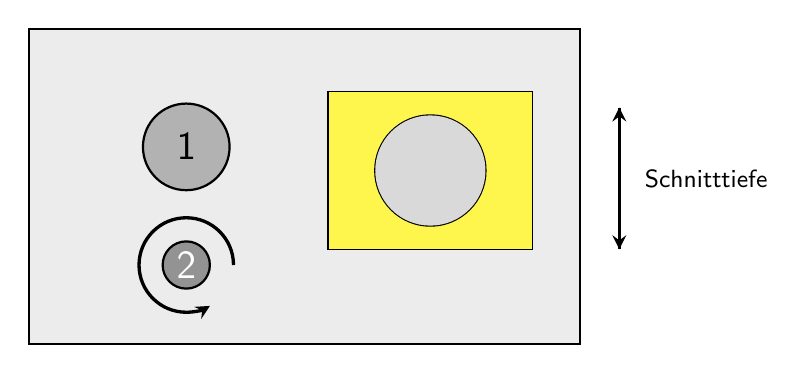
\begin{tikzpicture}[font=\Large,>=stealth]
% Frontplatte
\fill[gray!15] (0,0) rectangle (7,4); \draw[thick] (0,0) rectangle (7,4);
\fill[yellow!70] (3.8,1.2) rectangle (6.4,3.2); \draw (3.8,1.2) rectangle (6.4,3.2);
% große Verstellschraube 1
\fill[gray!60] (2,2.5) circle (0.55); \draw[thick] (2,2.5) circle (0.55); \node at (2,2.5) {1};
% kleine Verstellschraube 2
\fill[gray!85] (2,1.0) circle (0.3); \draw[thick] (2,1.0) circle (0.3); \node[white] at (2,1.0) {2};
\draw[->,very thick] (2.6,1.0) arc (0:300:0.6);
% Sägeblatt oben/unten
\begin{scope}[shift={(5.1,2.2)}]
 \draw[thick] (0,0) circle (0.7); \fill[gray!30] (0,0) circle (0.7);
\end{scope}
\draw[->,very thick] (7.5,1.2) -- (7.5,3.0);
\draw[->,very thick] (7.5,3.0) -- (7.5,1.2);
\node[right] at (7.7,2.1) {\small Schnitttiefe};
\end{tikzpicture}
\end{document}
